\chapter{Microsoft Teams}\label{teams1}  


La suite Microsoft comporte plusieurs applications qui possèdent des fonctionnalités différentes. En particulier, on notera les applications suivantes :\\

\begin{itemize}
\item \textit{Word} - est un éditeur de traitement de texte.
\item \textit{Excel} - est un tableur offrant une organisation visuelle des données et des outils d'analyse de contenu.
\item \textit{PowerPoint} - permet de créer des présentations.
\item \textit{Outlook} - est un outil de gestion des e-mails proposant un calendrier.
\item \textit{OneNote} - est un éditeur de prises de notes.
\item \textit{OneDrive} - est un cloud permettant de stocker des données sur des serveurs distants.
\item \textit{Teams} - est un outil centralisé permettant le travail collaboratif. Il gère notamment l'accès à OneNote, OneDrive ainsi qu'à la messagerie instantanée et Ourlook.
%\item \textit{Access} - est un gestionnaire de bases de données permettant la création d'applications commerciales.
%\item \textit{Edge} - est un navigator permettant l'accès à Internet.
%\item \textit{Skype} - est un gestionnaire de communication pour les appels et le chat.
%\item \textit{Sway} - est un outil de création de rapports et de newsletters interactives.
\end{itemize} 


% CONNEXION A OFFICE
\section{Connexion à Office 365 et Teams}

Ouvrez le navigateur internet de votre choix ou Safari et entrez l'URL suivante: \url{www.office.com}. Cliquez sur \texttt{Connexion}.

\begin{figure}[H]
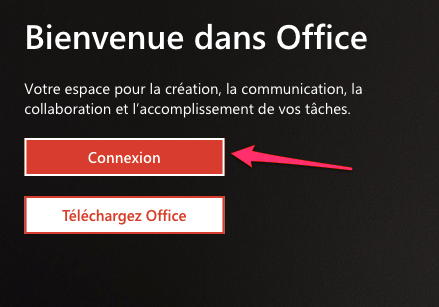
\includegraphics[width=5cm]{./images/teams/ecran_office_com_crop}
\centering
\end{figure}

Vous arrivez sur l'écran de connexion de \emph{Microsoft Office} en ligne. Entrez votre adresse mail de l'école (qui se termine donc par \textit{@florimont.ch}).

\begin{figure}[H]
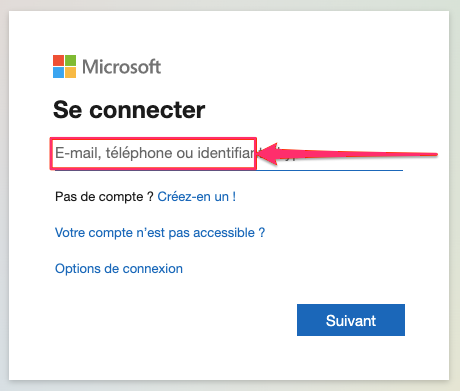
\includegraphics[width=5cm]{./images/teams/ecran_connexion_office_com_crop}
\centering
\end{figure}

Vous êtes alors redirigé vers la page d'identification de l’école. Entrez votre mot de passe. (l'adresse mail est déjà entrée, mais vous pouvez la modifier au cas où vous avez fait une erreur lors de l'étape précédente.)

\begin{figure}[H]
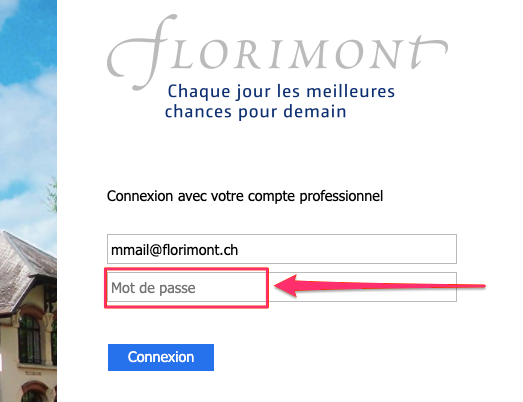
\includegraphics[width=5cm]{./images/teams/ecran_connexion_florimont_crop}
\centering
\end{figure}

Il se peut qu'on vous demande si vous voulez rester connecté. Si vous comptez travailler longtemps sur cette session, il vaut mieux accepter.\\

En revanche, si le navigateur vous propose d'enregistrer votre mot de passe, il est recommandé de refuser (soit en fermant la fenêtre, soit en choisissant \texttt{Jamais}). Si vous vous connectez depuis votre ordinateur personnel, il peut être pratique de permettre au navigateur de se souvenir de mots de passe, mais ce n'est jamais une bonne idée sur un ordinateur partagé ou d'emprunt.\\

Le site vous proposera peut-être de télécharger l’application. Cliquez alors sur \texttt{Utiliser l’application web à la place}.\\

Alternativement, sur certains navigateurs (comme Safari), vous devrez télécharger l'application de bureau Teams. Cliquez sur \texttt{Télécharger l'application} pour continuer.

\begin{figure}[H]
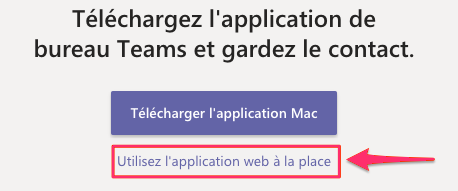
\includegraphics[width=6cm]{./images/teams/ecran_installer_teams_crop}
\centering
\end{figure}

Vous arrivez sur la page de téléchargement de l'application. Cliquez sur \texttt{Download Teams}, sous le logo de la pomme, pour télécharger l'application pour Mac.\\

Vous êtes à présent dans votre espace \emph{Office}. Sur la gauche, choisissez l'icône \emph{Teams}.

\begin{figure}[H]
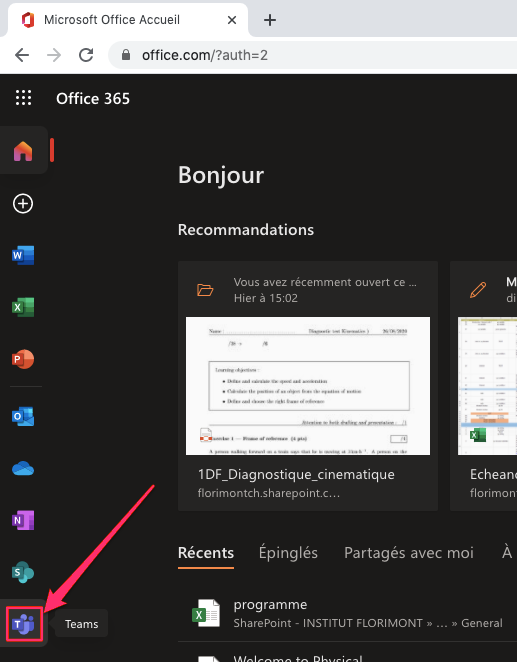
\includegraphics[width=5cm]{./images/teams/ecran_accueil_office_crop}
\centering
\end{figure}

Félicitations, vous arrivez sur la page d'accueil de votre session \emph{Teams}.




% UTILISATION DE LA PUBLICATION
\section{Utilisation de la Publication}

La messagerie instantanée proposée pour chaque équipe doit permettre aux élèves et aux enseignants de communiquer en dehors de l'école dans un cadre qui reste strictement scolaire. Ainsi les messages personnels n'ont aucune raison d'être sur \emph{Teams}. Il vous appartient donc de mesurer vos propos lorsque vous utilisez la messagerie instantanée. Ainsi, toute forme d'insulte ou de critique envers un membre de la classe ou une personne extérieure est à proscrire. Le modérateur de chaque équipe est son enseignant responsable.\\

Pour utiliser la messagerie, il suffit de vous rendre sur l'onglet \texttt{Publications}

\begin{figure}[H]

\includegraphics[width=9cm]{./images/teams/publications}
\centering
\end{figure}

puis de rédiger du texte à l'intérieur du champ \texttt{Démarrer une conversation}. Utilisez @ pour mentionner un contact, ce qui signifie qu'une notification sera adressée à cette personne. Attention donc de ne pas mentionner un contact inutilement.

\begin{figure}[H]
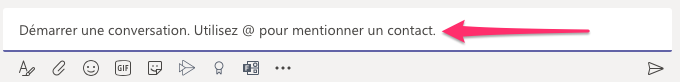
\includegraphics[width=9cm]{./images/teams/publications2}
\centering
\end{figure}

Il ne vous reste plus qu'à cliquer sur l'icône 
\includegraphics[width=0.7cm]{./images/teams/envoi_message} pour envoyer votre message.

\begin{figure}[H]
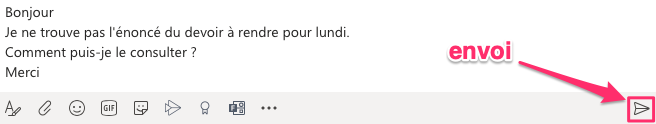
\includegraphics[width=9cm]{./images/teams/publications3}
\centering
\end{figure}





% CONSULTER ET TELECHARGER UN DOCUMENT
\section{Consulter et télécharger un document}

Vous devrez souvent chercher des documents mis en ligne par vos enseignants. Pour faire cela, sélectionnez l'onglet \texttt{Fichiers}, en haut.

\begin{figure}[H]
	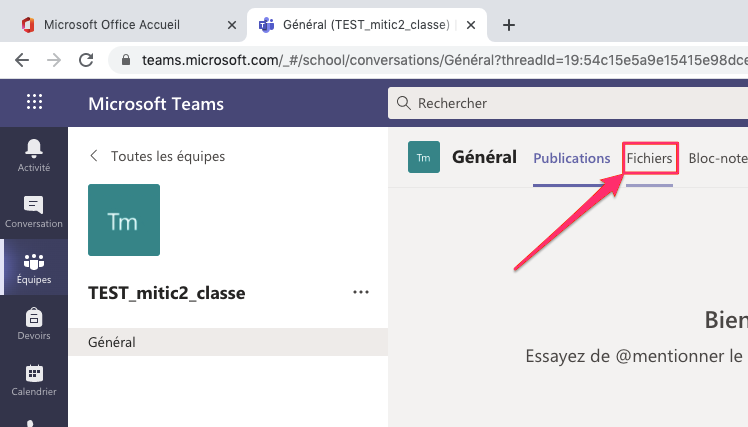
\includegraphics[width=8cm]{./images/teams/accueil_classe_crop}
	\centering
\end{figure}

Les fichiers que vos enseignants mettront à votre disposition seront la plupart du temps rangés dans un dossier. Dans cet exemple, il n'y a qu'un dossier, \texttt{Support de cours}. Cliquez dessus pour l'ouvrir.

\begin{figure}[H]
	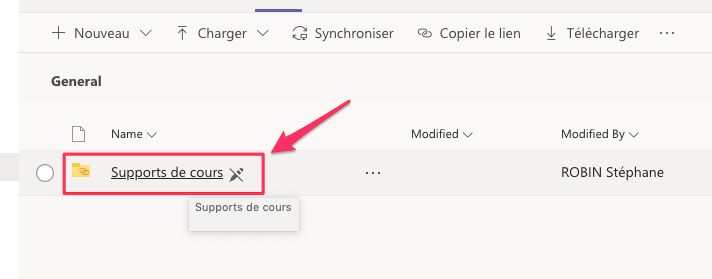
\includegraphics[width=9cm]{./images/teams/ouvrir_dossier_crop}
	\centering
\end{figure}

Vous trouverez dans ce dossier le fichier que votre professeur vous demandera de consulter. Pour le lire, il suffit de cliquer dessus.

\begin{figure}[H]
	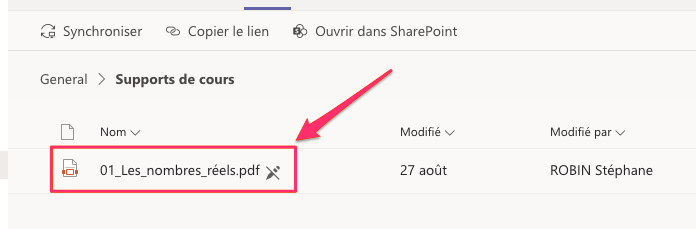
\includegraphics[width=9cm]{./images/teams/ouvrir_fichier_crop}
	\centering
\end{figure}

Vous pouvez à présent consulter le document, mais pas le modifier. Vous pouvez le télécharger pour en garder une copie sur votre ordinateur et éventuellement le modifier par la suite en cliquant sur les trois petits points en haut, puis sur \texttt{Télécharger}. Une copie du document apparait alors dans votre dossier \texttt{Téléchargement}.\\

Une fois cela fait, vous pouvez quitter cette page pour revenir à l'affichage du dossier en cliquant sur \texttt{Fermer}.
\newpage
\begin{figure}[H]
	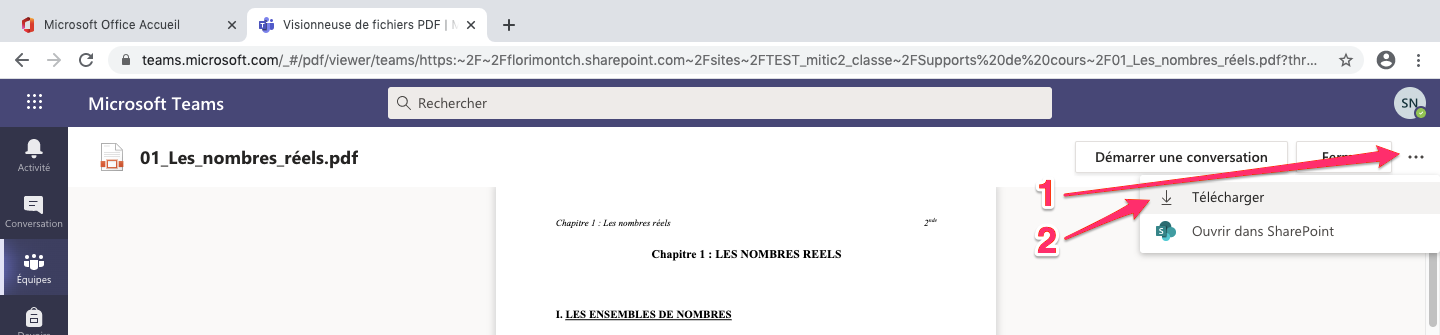
\includegraphics[width=9cm]{./images/teams/telecharger_document_crop}
	\centering
\end{figure}

Il est également possible de télécharger un document depuis la vue du dossier. Il existe plusieurs manières de faire cela. La première consiste à cliquer sur les trois petits points à côté du nom du document, puis sur \texttt{Télécharger}.

\begin{figure}[H]
	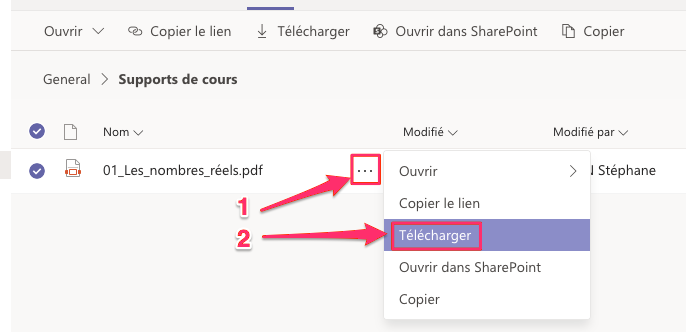
\includegraphics[width=9cm]{./images/teams/telecharger1_crop}
	\centering
\end{figure}

Alternativement, vous pouvez cliquer sur le rond à gauche du nom de fichier pour le sélectionner. Cliquez ensuite sur \texttt{Télécharger}, en haut pour télécharger ce fichier. Cette dernière méthode est très pratique si vous désirez télécharger plusieurs fichiers d'un coup, car il suffit alors de les sélectionner puis de cliquer sur \texttt{Télécharger} pour les récupérer en même temps.

\begin{figure}[H]
	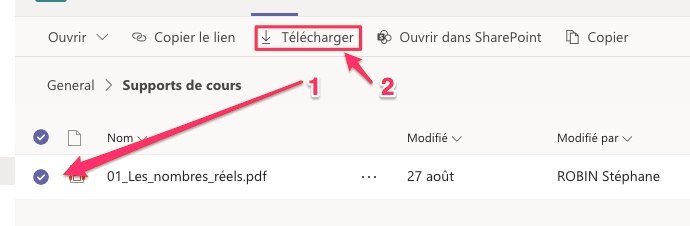
\includegraphics[width=9cm]{./images/teams/telecharger2_crop}
	\centering
\end{figure}



% DEPOSER UN DEVOIR
\section{Les devoirs}

\subsection{Consulter le sujet d'un devoir en pièce jointe}\label{consulterDevoir}
Pour consulter les devoirs déposés par votre enseignant, il faut choisir \texttt{2 de plus} dans la barre de menus du haut de page, puis sélectionner \texttt{Devoirs}.

\begin{figure}[H]
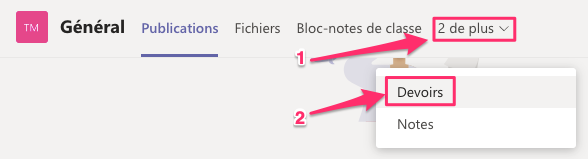
\includegraphics[width=9cm]{./images/teams/devoir1}
\centering
\end{figure}

La page qui s'affiche maintenant fait le bilan de ce qui a déjà été fait et des devoirs proposés par votre enseignant. En cliquant sur \texttt{Rédaction} vous pourrez accéder au devoir.

\begin{figure}[H]
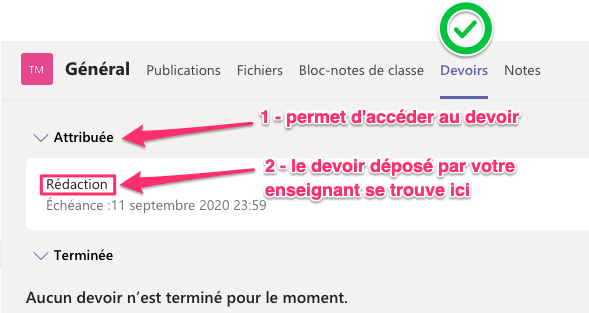
\includegraphics[width=9cm]{./images/teams/devoir2}
\centering
\end{figure}

Vous obtenez alors l'écran suivant

\begin{figure}[H]
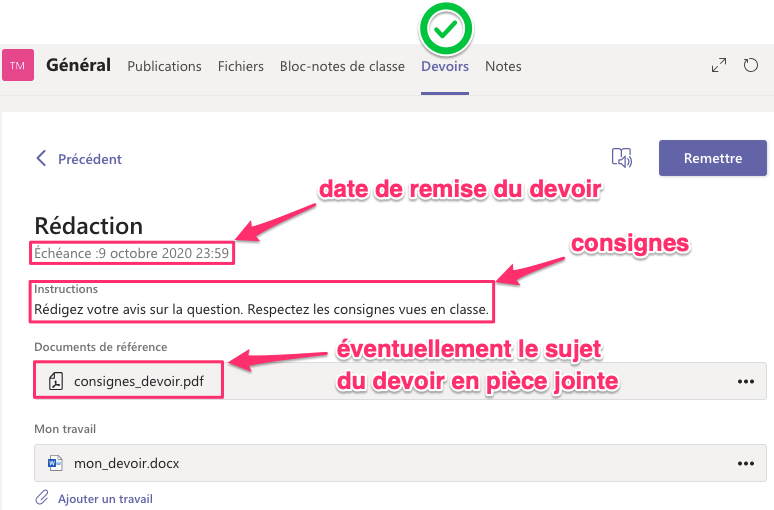
\includegraphics[width=9cm]{./images/teams/devoir3}
\centering
\end{figure}

Il est maintenant possible de consulter le sujet en sélectionnant l'icône 
\includegraphics[width=0.7cm]{./images/teams/pointilles} qui vous offre le choix entre une lecture en ligne ou un téléchargement

\begin{figure}[H]
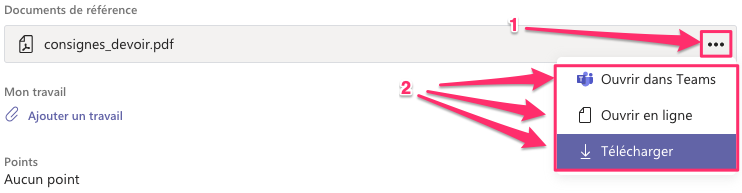
\includegraphics[width=9cm]{./images/teams/choix_pointilles}
\centering
\end{figure}

% REMETTRE SON DEVOIR
\subsection{Remettre son devoir}\label{TeamsRemettreDevoir}

Pour remettre votre devoir, il faut d'abord cliquer sur l'onglet \texttt{Ajouter un travail}. 

\begin{figure}[H]
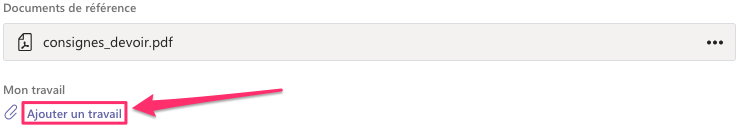
\includegraphics[width=9cm]{./images/teams/ajout}
\centering
\end{figure}

S'ouvre alors une fenêtre qui vous permet de rechercher votre document à partir d'un dossier local relatif à votre ordinateur, à partir du \emph{OneDrive} ou encore à partir d'une autre équipe.

\begin{figure}[H]
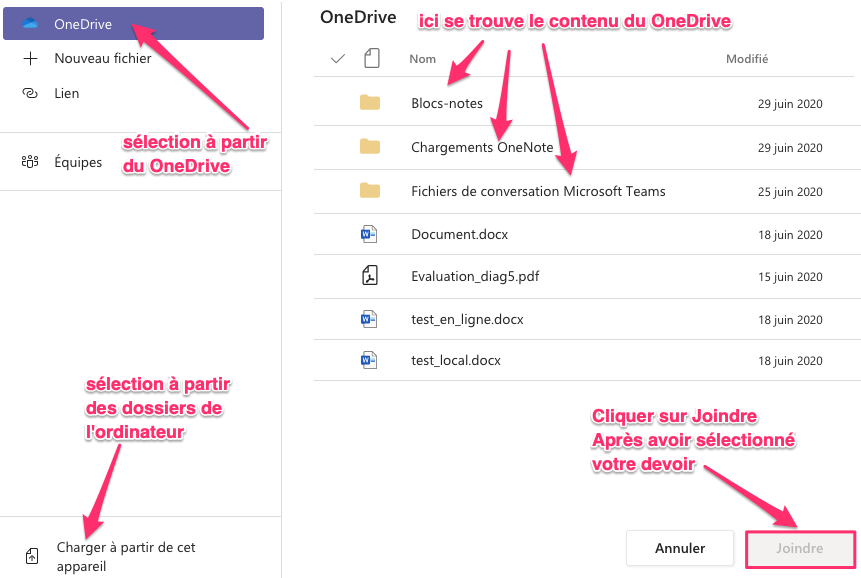
\includegraphics[width=11cm]{./images/teams/selection_devoir}
\centering
\end{figure}

Une fois votre devoir à remettre sélectionné, il suffit de cliquer sur \texttt{Joindre}. A ce stade, votre devoir n'est pas encore enregistré. Il faut maintenant choisir \texttt{Terminé} pour l'enregistrer.

\begin{figure}[H]
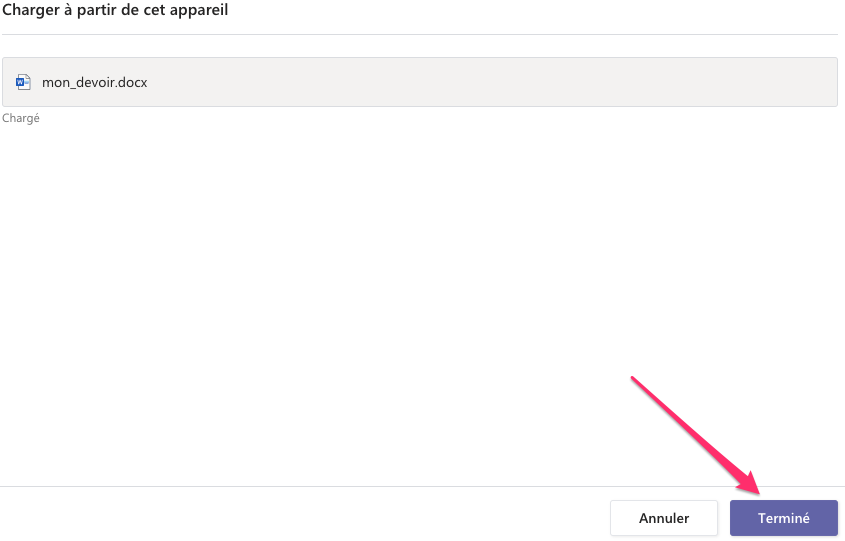
\includegraphics[width=9cm]{./images/teams/ajout2}
\centering
\end{figure}

Vous pouvez également ajouter un autre travail, vous pouvez également télécharger votre devoir afin de vérifier son contenu. Vous pouvez également supprimer votre travail.

\begin{figure}[H]
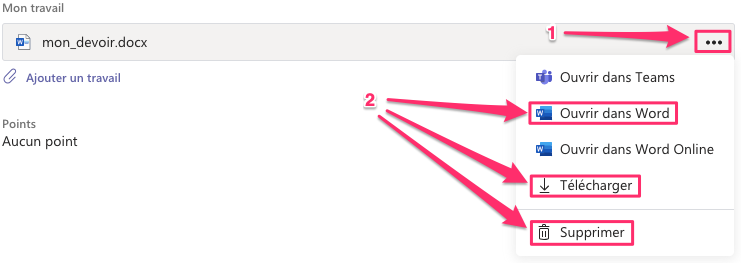
\includegraphics[width=9cm]{./images/teams/ajout3}
\centering
\end{figure}

Attention, votre devoir n'est pas encore remis. il faut maintenant choisir l'onglet \texttt{Remettre} pour valider l'envoi de votre devoir. 

\begin{figure}[H]
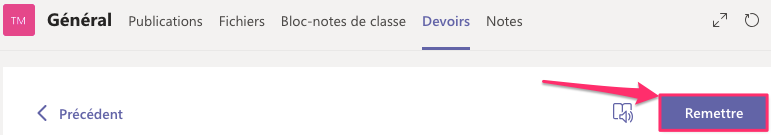
\includegraphics[width=9cm]{./images/teams/ajout4}
\centering
\end{figure}


% ACCEDER A MON CARNET
\section{Accéder à mon bloc-note}

Certains de vos enseignants mettront à votre disposition un bloc-note de classe. C'est un outil très pratique qui permet de prendre des notes et de modifier des fichiers mis à votre disposition, directement depuis \emph{Teams}.\\

Pour accéder au carnet de classe, cliquez sur \texttt{Bloc-notes de classe}, en haut de la page de la classe.

\begin{figure}[H]
	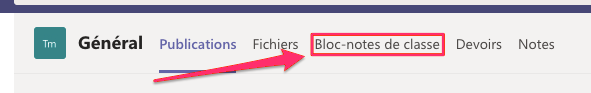
\includegraphics[width=9cm]{./images/teams/acces_bloc_notes_crop}
	\centering
\end{figure}

S'ouvre alors la page d'accueil du bloc-notes. Votre enseignant l'aura probablement adaptée à son cours, elle ne ressemblera donc pas forcément à l'image ci-dessous.

\begin{figure}[H]
	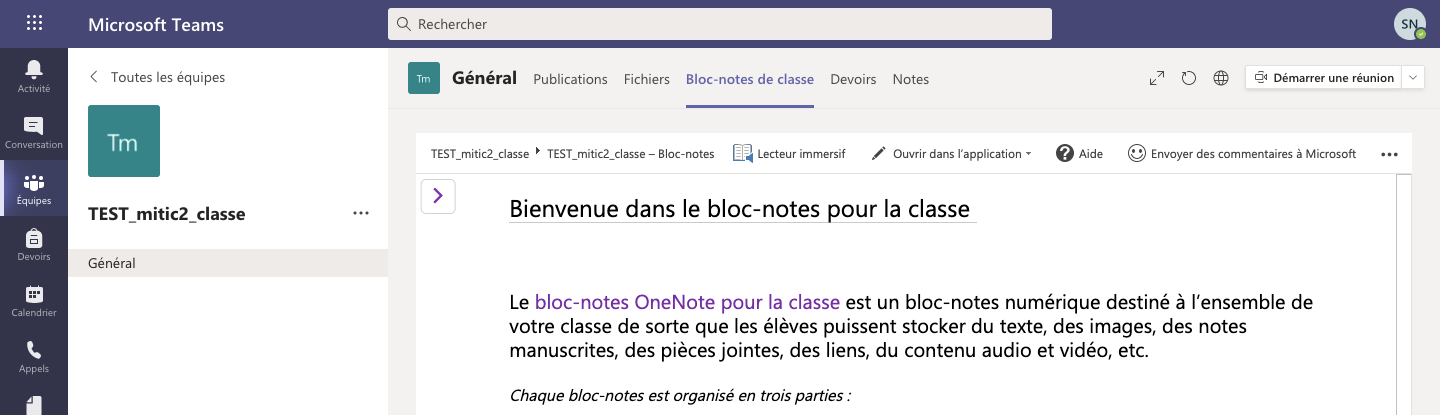
\includegraphics[width=11cm]{./images/teams/ouvrir_menu_bloc_notes_crop}
	\centering
\end{figure}

Cliquez sur la flèche en haut à gauche de l'espace de travail pour ouvrir la liste des bloc-notes. Une section à votre nom apparait, en bas de la liste. Il s'agit d'un espace personnel dans lequel vous pouvez écrire ce que vous voulez, que ce soit pour modifier des fichiers ou prendre des notes. Cliquez sur votre nom pour afficher des sous-sections.

\begin{figure}[H]
	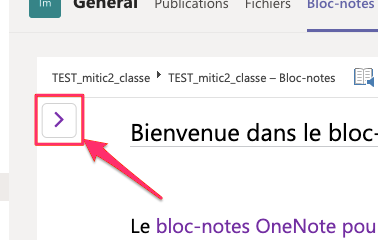
\includegraphics[width=6cm]{./images/teams/ouvrir_liste_dossiers_docs_crop}
	\centering
\end{figure}

Ouvrez la page sans titre, dans la sous-section \texttt{Documents}. Ecrivez le titre de votre document. Vous verrez que le titre sera mis à jour dans la liste de documents, à gauche. Si votre liste de sections et documents s'est refermée, il suffit de cliquer sur la flèche, comme tout à l'heure, pour l'afficher à nouveau.\\

Vous pouvez maintenant écrire du texte, ajouter des images, ou modifier ce document comme vous le souhaitez.\\

Si vous souhaitez ajouter une nouvelle page, vous pouvez cliquer sur \texttt{+ Page}, en bas. Renommez la nouvelle page en écrivant un titre comme vous venez de le faire.

\begin{figure}[H]
	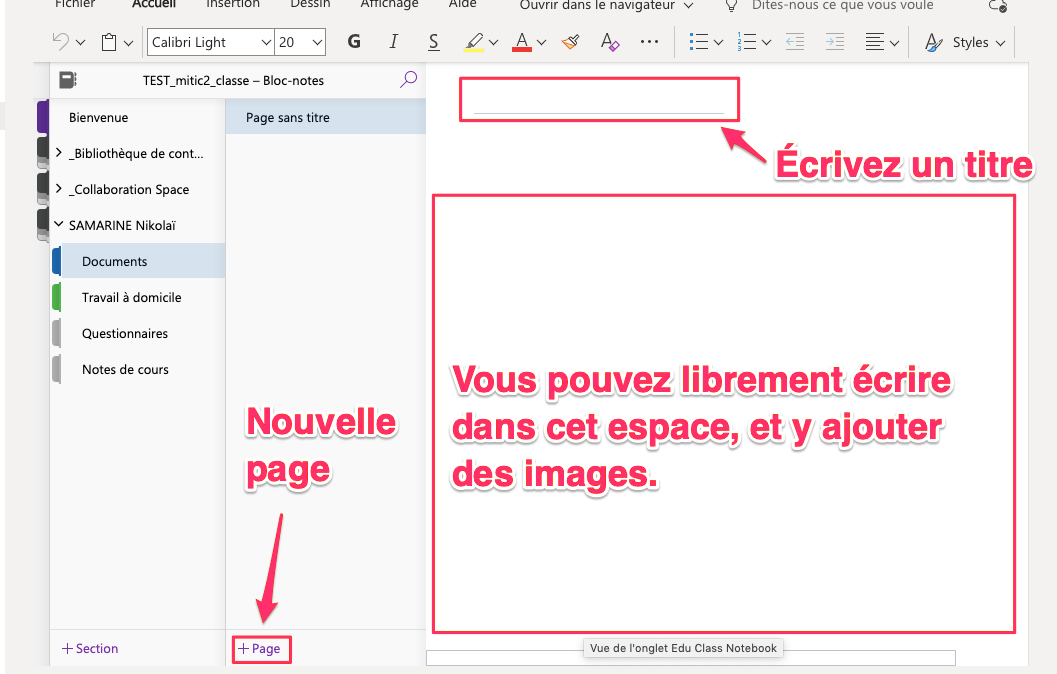
\includegraphics[width=10cm]{./images/teams/sous_section_documents_crop}
	\centering
\end{figure}

En ajoutant et modifiant ainsi des pages, vous allez pouvoir prendre des notes et y accéder via divers appareils, que ce soit depuis la maison ou l'école.

% REJOINDRE UNE VISIO CONFERENCE
\section{Rejoindre une visio-conférence}

Lorsque vous devez assister à un cours à distance, il est nécessaire de rejoindre une visio-conférence déjà commencée. Pour cela, dans l'onglet \texttt{Publications}, vous aller trouver une invitation pour participer à une visio-conférence déjà ouverte

\begin{figure}[H]
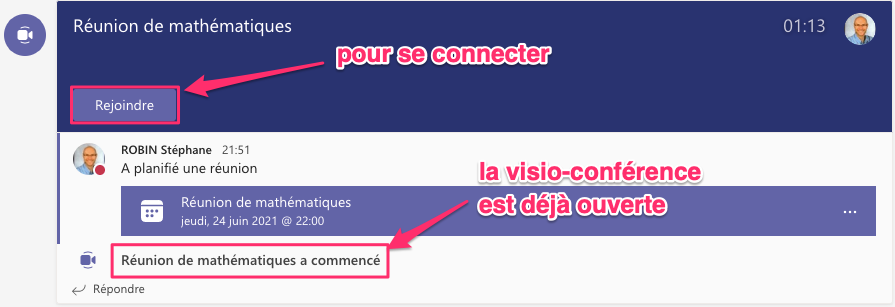
\includegraphics[width=12cm]{./images/teams/video3.png}
\centering
\end{figure}

Attention, si vous sélectionnez \texttt{Demarrer une réunion}, vous allez créer une nouvelle visio-conférence et non pas rejoindre la visio-conférence déjà programmée pour votre cours.

\begin{figure}[H]
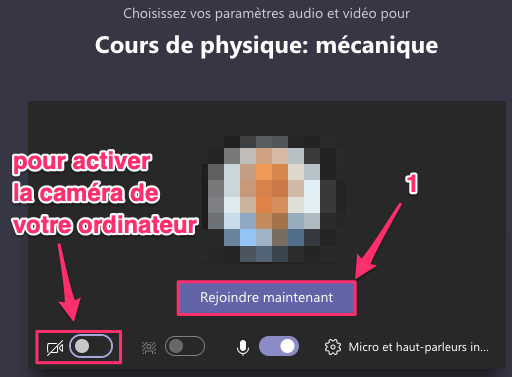
\includegraphics[width=7cm]{./images/teams/video2}
\centering
\end{figure}





% APPARENCE DE LA PAGE D'ACCUEIL
\section{Pour aller plus loin}
\subsection{Apparence de la page d'accueil}

La page d'accueil de \emph{Teams} se présente sous forme d'une liste d'équipes

\begin{figure}[H]
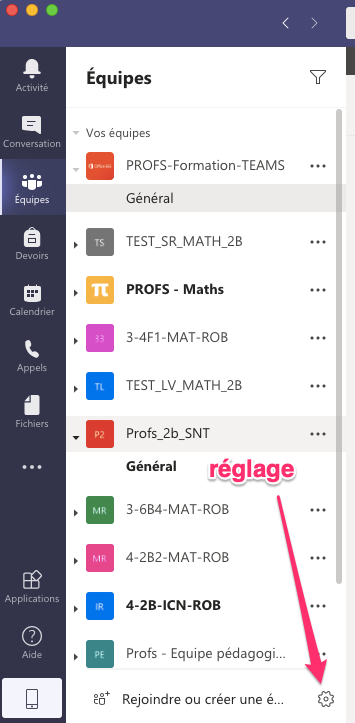
\includegraphics[width=4cm]{./images/teams/accueil_liste}
\centering
\end{figure}

\newpage
ou sous forme d'une grille d'équipes 

\begin{figure}[H]
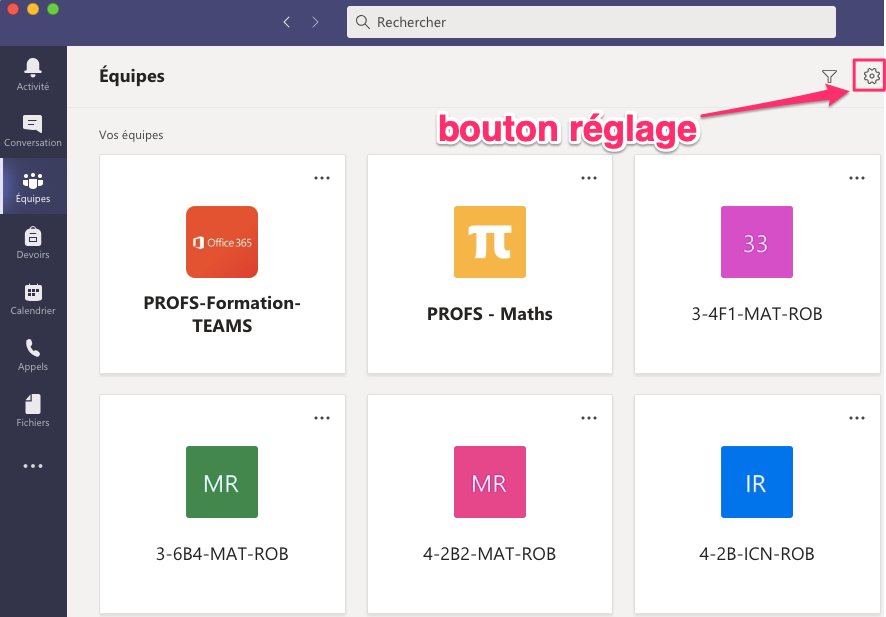
\includegraphics[width=7cm]{./images/teams/accueil_grille}
\centering
\end{figure}

Pour passer d'une forme à l'autre, il faut cliquer sur l'icône 
\includegraphics[width=0.8cm]{./images/teams/bouton_parametres}, choisir \texttt{Changer d'affichage} dans le menu déroulant, comme dans l'exemple illustré ci-dessous :

\begin{figure}[H]
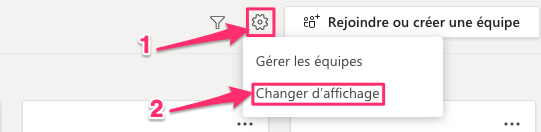
\includegraphics[width=9cm]{./images/teams/changement_liste}
\centering
\end{figure}

Il faut ensuite sélectionner le type d'affichage souhaité entre \texttt{Grille} et \texttt{Liste}

\begin{figure}[H]
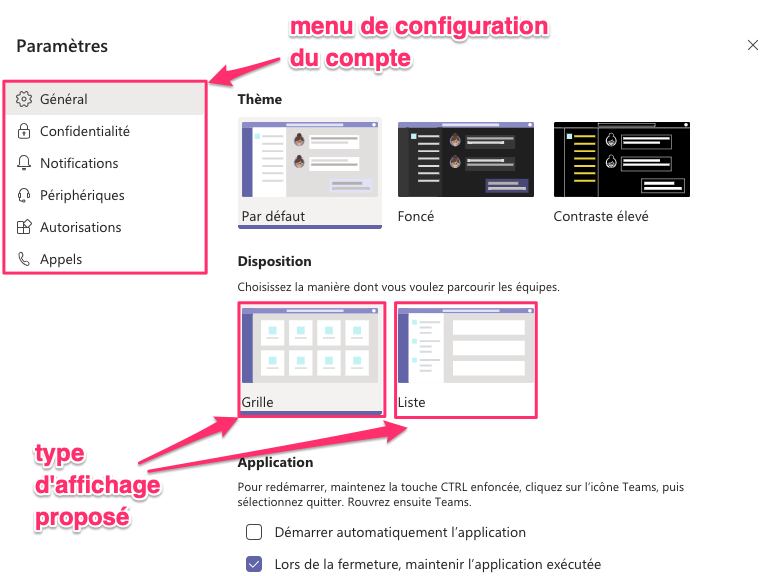
\includegraphics[width=9cm]{./images/teams/choix_parametre}
\centering
\end{figure}

 Pour entrer maintenant dans votre équipe, il suffit de cliquer sur l'icône correspondante

\begin{figure}[H]
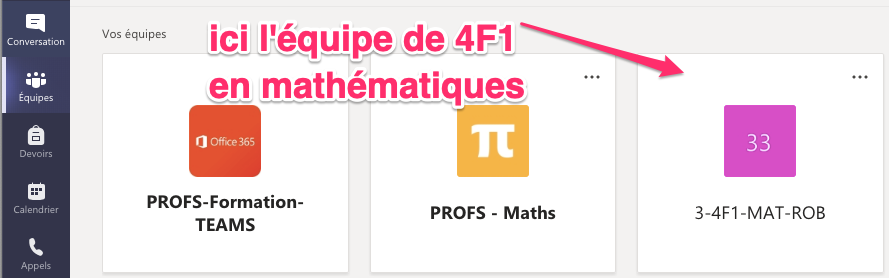
\includegraphics[width=7.5cm]{./images/teams/entree_classe}
\centering
\end{figure}

\subsection{Activité d'exploration de Teams}

C'est à vous de montrer à quel point vous connaissez bien \emph{Teams} ! Des indices permettant de retrouver un mot mystère se sont cachés dans \emph{Teams}. Essayez de retrouver tous les indices, et reconstituez le mot mystère. Chaque indice vous indique aussi comment trouver le suivant !\\

Le premier indice a été repéré sur l'espace Publications de la page de votre cours. \\Bonne chance !

%\prof{
\subsection*{Préparation de l'activité pour les enseignants}

Pour cette activité, vous devez préparer l’espace \emph{Teams} de votre classe pour que les élèves puissent trouver les indices leur permettant d’arriver au bout. Voici la liste de ce qu’il faut faire :
\begin{itemize}
\item Dans les \texttt{Fichiers} de la classe, dans le \texttt{Support de cours}, ajouter un fichier \emph{Word} nommé \texttt{indice\_mot\_mystere.docx} et dont le contenu est le texte suivant : \emph{Vous avez trouvé la lettre « M » ! La prochaine vous sera révélée dès que vous aurez rejoint une visio-conférence…}

\item Créer une page dans le \texttt{Bloc-notes} de la classe (ou en distribuer une à tous les élèves) dont le titre est "Indice pour le mot mystère" et dont le contenu est le texte suivant : \emph{Une autre lettre est le « S ». La prochaine lettre se trouve dans la pièce jointe du devoir que vous devez remettre.}

\item Créer un devoir, où les élèves rendront un document avec leur mot. Ce devoir doit avoir une pièce jointe, un document PDF nommé \texttt{informations\_devoir.pdf} et dont le contenu est le texte suivant : \emph{Bravo, vous avez trouvé la lettre « A ». Maintenant, vous devez former un mot avec les lettres que vous avez trouvées et le rendre comme un devoir. Attention! Vous ne pouvez utiliser chaque lettre qu'une fois, et ne devez utiliser que celles que vous avez trouvées!}

\item Imprimer un document sur lequel on peut clairement lire ceci: \emph{Avec ce « T », ça fait déjà 3 lettres ! La prochaine se trouve dans une feuille du Bloc-notes.} et l'imprimer sur une page que vous allez replier de manière à pouvoir la faire tenir debout. Ouvrez une visioconférence et positionnez votre caméra de manière à ce qu'on puisse lire le texte sur le document imprimé.

\item Créer une nouvelle publication (ou annonce) avec comme contenu le texte suivant: \emph{La première lettre à trouver est le « E » et vous trouverez la prochaine dans un fichier du dossier} \texttt{Support de cours}.
\end{itemize}

%}
